\chapter{\label{chap:spelunkbots}SpelunkBots}

Utilizando o código-fonte de Spelunky, Daniel Scales e Thomas Thompson, da
Universidade de Derby no Reino Unido, criaram o
\textit{SpelunkBots}\cite{SPELUNKBOTSPAPER}, um
\textit{framework} que permite a programação de \textit{bots} para o jogo
Spelunky. Um dos objetivos dos criadores é utilizar a aplicação para criar uma
competição de inteligência artificial para o jogo.

A \textit{API} possibilita que o desenvolvedor resgate informações de objetos
estáticos e dinâmicos contidos no ambiente do jogo, como o terreno, a
posição de tesouros, armadilhas e inimigos. Contudo, o objetivo da \textit{API}
disponibilizada por SpelunkBots é fazer com que a informação recebida pelo
\textit{bot} se assemelhe ao máximo com a percepção de um jogador humano.  Para
tal, o \textit{framework} implementa um sistema de \textit{fog of war},
limitando o conhecimento do ambiente que pode ser obtido pela inteligência
artificial. Para objetos estáticos, uma vez que o jogador visualizou o objeto,
ele poderá receber informações sobre ele permanentemente. Para objetos
dinâmicos, o \textit{bot} só poderá receber informações sobre eles se os mesmos
estiverem sendo visualizados por ele. A figura \ref{fig:spelunkbots-fow} ilustra
um exemplo de funcionamento do sistema, onde as áreas apresentadas na coloração
cinza e marcadas com o valor ``1'' representam pontos sobre os quais o
\textit{bot} não tem conhecimento algum, pois ainda não explorou a área
que o permite que sejam revelados os elementos do jogo que se encontram
nesses pontos.

\begin{figure}[htb!]
\centering
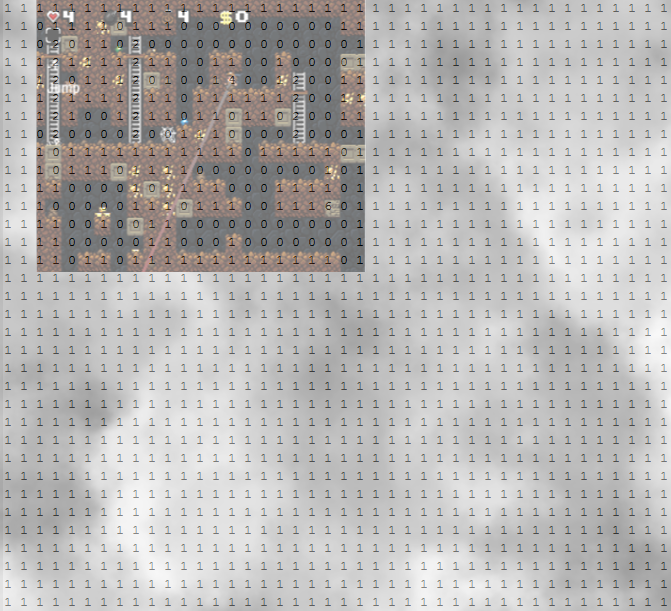
\includegraphics[width=.65\textwidth]{fig/spelunkbots-fow.png}
\caption {\label{fig:spelunkbots-fow}Visualização do sistema de \textit{fog of
war} demonstrando a diferença de informação recebida de elementos dentro e fora
do campo de visão do jogador.}
\end{figure}

\section{Utilização da \textit{API}}

É possível desenvolver \textit{bots} que fazem uso da \textit{API}
utilizando a linguagem GML (sigla para \textit{Game Maker Language}) ou
através da linguagem C++, ficando a critério do desenvolvedor a escolha da
linguagem. A única restrição que existe quanto ao uso de C++ dá-se no fato
de que a linguagem necessita de um processo de compilação através de uma
ferramenta externa, não sendo gerenciada diretamente pelo \textit{Game
Maker}. (COLOCAR FIGURINHA AQUI)

A \textit{API} permite uma interação completa com o jogo através do uso
das variáveis expostas pelo
\textit{framework}\footnote{http://spelunkbots.com/wp-content/uploads/2015/02/SpelunkBots-API-A-Getting-Started-Tutorial.pdf}.
Com essas variáveis é possível fazer o controle da movimentação do bot, bem
como identificar o tipo de terreno em que se está pisando e os inimigos que
aparecem em seu campo de visão. Além disso, também são disponibilizadas
informações sobre as armadilhas que podem atrapalhar o jogador. Por fim,
existem variáveis que permitem um melhor controle das informações relativas ao
\textit{bot}, como o posicionamento no eixo X e no eixo Y, se o \textit{bot}
encontra-se virado para a esquerda ou para a direita, entre outros.

\begin{itemize}
    \item Motivação: citar os porquês de ter sido criado (citar o paper do
        Scales e do Thompson \cite{SPELUNKBOTSPAPER}), bem como as possíveis
        competições que surgem a partir da criação desses (só citar mesmo,
        entrar em detalhes no capítulo específico).
    \item Explicar sobre a API e suas características ``interessantes''
        (\textit{fog war} com figura e explicações)
    \item Explicar como é feito o uso da API por um desenvolvedor (GML ou
        C++). Talvez seja interessante explicar alguma coisa das DLLs,
        para o caso de usar C++ (aqui vai uma figurinha bacana mostrando a
        ``arquitetura'')
    \item Interação com o Jogo
        \footnote{http://spelunkbots.com/wp-content/uploads/2015/02/SpelunkBots-API-A-Getting-Started-Tutorial.pdf}
    \begin{itemize}
        \item Explicar as variáveis globais de movimentação
        \item Explicar as variáveis globais do terreno (talvez vale
            colocar figuras aqui)
        \item Explicar as variáveis globais dos obstáculos (inimigos vêm aqui)
        \item Explicar as variáveis globais referentes aos objetos
        \item Explicar as variáveis globais referentes ao player
    \end{itemize}
\end{itemize}
